\documentclass[a4paper,12pt]{article}

%Class
	%\documentclass[a4paper,12pt]{article}

%Packages
	\usepackage{amsmath}					% Standard maths
	\usepackage{amssymb}					% Standard maths
	\usepackage{amsthm}						% Standard maths
	\usepackage{thmtools, thm-restate}% Theorem styles
	\usepackage{mathtools}
	\usepackage[newzealand]{babel}% Date/time in British format (yes, I know it says NZ)
	\usepackage{datetime}					% Date/time
	\usepackage{multirow}					% For stacked subscripts
	\usepackage{xcolor}						% For colour!
	\usepackage[normalem]{ulem}		% For strikeout
	\usepackage{isomath}
	\usepackage{fancyhdr}					% For the headers
	\usepackage{mfirstuc}					% For the headers
	\usepackage[hmargin=1in,top=0.8in,bottom=1in]{geometry} % Page margins more reasonable
	\usepackage{graphicx}					% For including graphics
	%\usepackage{float}						% For something
	\usepackage{enumitem}					% For numbering tweaks
	\usepackage{pgfplots}
	\usepackage[margin=15pt,font={footnotesize},labelfont=bf,format=hang]{caption}
\usepackage[margin=15pt,font={footnotesize},labelfont=bf,format=hang]{subcaption}
	\usepackage{url}
	\usepackage[hidelinks]{hyperref}	% For hyperlinks
	\usepackage{breakurl}
	\usepackage{cleveref}
	\usepackage[scaled=.92]{helvet}
	\newbool{show_question}
	\newbool{show_solution}
	\newcommand{\solutioninheading}{\ifbool{show_solution}{: SOLUTIONS}{}}
	\usepackage{pgfplots}
\newcommand{\ep}{\varepsilon}

\makeatletter 
\newcommand\mynobreakpar{\par\nobreak\@afterheading} 
\makeatother

    \newcommand{\question}[3]{
    	\item \textbf{#1} \mynobreakpar \nobreak \medskip % Title
    	%
    	\ifbool{show_question}{\nobreak#2}{} % Question
    	%
    	%
    	\ifbool{show_question}{\ifbool{show_solution}{\par\medskip\textbf{Solution:}}{}}{} % Both
    	\ifbool{show_solution}{#3}{} % Answer
    }			

%MATHEMATICAL SHORTCUTS
%Two and three-part definitions
	\newcommand{\twopartdef}[4]
	{	\left\{
			\begin{array}{ll}
				#1 & \mbox{if } #2 \\
				#3 & \mbox{if } #4
			\end{array}
		\right.}
%	\newcommand{\threepartdef}[6]
%	{	\left\{
%			\begin{array}{ll}
%				#1 & \mbox{if } #2 \\
%				#3 & \mbox{if } #4 \\
%				#5 & \mbox{if } #6
%			\end{array}
%		\right.}
%Blackboard bold	
	\newcommand{\N}{{\mathbb N}} 
	\newcommand{\R}{{\mathbb R}} 
	\newcommand{\C}{{\mathbb C}} 
	%Curly letters
%	\newcommand{\E}{{\mathcal E}}	
%	\newcommand{\F}{{\mathcal F}} 
%	\newcommand{\Null}{{\mathcal N}} 
%	\newcommand{\R}{\mathcal{R}} 
%	\newcommand{\Z}{\mathcal{Z}} 
%Uprights
	\newcommand{\D}{{\mathrm D}}
	\renewcommand{\d}{{\mathrm d}}
%Easy Greeks
%	\def\a{\alpha}
%	\def\g{\gamma}
%	\newcommand{\e}{{\varepsilon}}
%	\newcommand{\la}{{\lambda}}  
%	\newcommand{\om}{{\Omega}}
	\renewcommand{\epsilon}{\varepsilon}
	
%Vector operators
	\def \p {\partial}
	\newcommand{\del}{{\nabla}}
	\newcommand{\grad}{{\nabla}}
    \newcommand{\vdel}{\boldsymbol{\nabla}}
    \newcommand{\vgrad}{\boldsymbol{\nabla}}
    \newcommand{\vnabla}{\boldsymbol{\nabla}}
	\newcommand{\cross}{{\times}}
	\newcommand{\Lap}{{\nabla^2}} 
%Arrows
%	\newcommand{\goesto}[1]{\xrightarrow[#1]{}}
%hats
%	\newcommand{\nhat}{\widehat{\v{n}}}
%	\newcommand{\shat}{\widehat{\v{s}}}
	\renewcommand{\hat}{\widehat}
%Note to self
%	\newcommand{\note}[1]{[\textbf{\textsl{\MakeUppercase{#1}}}]}
	
%Stress tensor
%	\newcommand{\T}{\vg{\sigma}}

% Vectors, quaternions etc.
\renewcommand{\v}[1]{\mathbfit{#1}}      % Generic vector
\newcommand{\vc}[1]{\bm{\mathcal{#1}}}      % vector mathcal
\newcommand{\uv}[1]{\widehat{\mathbfit{#1}}}      % Generic unit vector
\newcommand{\q}[1]{\mathsfbfit{#1}}        % Generic quaternion
\renewcommand{\t}[1]{\mathsfbfit{#1}}	 % Generic tensor
\newcommand{\m}[1]{\mathsfbfit{#1}}	 % Generic matrix
\newcommand{\vu}[1]{\mathbf{#1}}         % Upright vector (for zero vector)
\newcommand{\qu}[1]{\mathbf{#1}}       % Upright quaternion (for zero quaternion)
\newcommand{\tu}[1]{\bm{\mathsf{#1}}}	 % Upright tensor (for zero tensor)

%Real and imaginary
\renewcommand{\Re}{\operatorname{Re}}
\renewcommand{\Im}{\operatorname{Im}}
	
%Non-dim numbers
%	\renewcommand{\Re}{\operatorname{Re}}
%	\newcommand{\Bi}{\operatorname{Bi}}
%	\newcommand{\Fo}{\operatorname{Fo}}
	
%Misc
\DeclareMathSymbol{\Delta}{\mathalpha}{operators}{1} % Keeps Delta upright
\DeclareMathSymbol{\Gamma}{\mathalpha}{operators}{0} % Keeps Gamma upright
	\newcommand{\cosec}{\operatorname{cosec}}
	\newcommand{\cosech}{\operatorname{cosech}}
	\newcommand{\sech}{\operatorname{sech}}
	\newcommand{\tr}{\operatorname{tr}}
	\newcommand{\erf}{\operatorname{erf}}
	\newcommand{\order}{\mathcal{O}}
%	\newcommand{\V}{\mathcal{V}} % 	CurlyV = (Bi V) / (1 + Bi)

% Differentiating 
\newcommand{\fd}[2]{\mathchoice{\frac{\d #1}{\d #2}}{\d #1/\d #2}{\d #1/\d #2}{\d #1/\d #2}}
\newcommand{\fdd}[2]{\mathchoice{\frac{\d^2 #1}{\d #2^2}}{\d^2 #1/\d #2^2}{\d^2 #1/\d #2^2}{\d^2 #1/\d #2^2}}
\newcommand{\fddd}[2]{\mathchoice{\frac{\d^3 #1}{\d #2^3}}{\d^3 #1/\d #2^3}{\d^3 #1/\d #2^3}{\d^3 #1/\d #2^3}}
\newcommand{\fdddd}[2]{\mathchoice{\frac{\d^4 #1}{\d #2^4}}{\d^4 #1/\d #2^4}{\d^4 #1/\d #2^4}{\d^4 #1/\d #2^4}}
\newcommand{\fdn}[3]{\mathchoice{\frac{\d^{#1} #2}{\d #3^{#1}}}{\d^{#1} #2/\d #3^{#1}}{\d^{#1} #2/\d #3^{#1}}{\d^{#1} #2/\d #3^{#1}}}
\newcommand{\pd}[2]{\mathchoice{\frac{\p #1}{\p #2}}{\p #1/\p #2}{\p #1/\p #2}{\p #1/\p #2}}
\newcommand{\pdd}[2]{\mathchoice{\frac{\p^2 #1}{\p #2^2}}{\p^2 #1/\p #2^2}{\p^2 #1/\p #2^2}{\p^2 #1/\p #2^2}}
\newcommand{\pddmixed}[3]{\frac{\p^2 #1}{\p #2 \p #3}}
\newcommand{\pddd}[2]{\frac{\p^3 #1}{\p #2^3}}
\newcommand{\pdn}[3]{\mathchoice{\frac{\p^{#1} #2}{\p #3^{#1}}}{\p^{#1} #2/\p #3^{#1}}{\p^{#1} #2/\p #3^{#1}}{\p^{#1} #2/\p #3^{#1}}}
	
	% Misc
\newcommand{\e}{\mathrm{e}}
\renewcommand{\i}{\mathrm{i}}
\newcommand{\dx}{\,\mathrm{d}x}
\newcommand{\dy}{\,\mathrm{d}y}
\renewcommand{\epsilon}{\varepsilon}
\renewcommand{\Re}{\operatorname{Re}}
\newcommand{\Four}{\mathcal{F}}

\newcommand{\mat}[4]{\begin{pmatrix}#1 & #2 \\ #3 & #4 \end{pmatrix}}

	%Column vectors
	\makeatletter
\newcommand\rcvector[2][\\]{\ensuremath{%
  \global\def\rc@delim{#1}%
    \negthinspace\begin{pmatrix}
      \rc@vector #2,\relax\noexpand\@eolst%
    \end{pmatrix}}}
\def\rc@vector #1,#2\@eolst{%
  \ifx\relax#2\relax
    #1
  \else
    #1\rc@delim
    \rc@vector #2\@eolst%
  \fi}
\makeatother

\newcommand{\colvec}{\rcvector}
\newcommand{\rowvec}{\rcvector}
\renewcommand{\binom}{\rcvector}
	
	%Colours
%	\newcommand{\orange}[1]{{\color{orange} #1 }}
%	\newcommand{\blue}[1]{{\color{blue} #1 }}

%Theorem styles
%	\declaretheoremstyle[headpunct={\:\:\:}, shaded={bgcolor={rgb}{0.9,0.9,0.9}, margin=5pt}]{problem}
%	\declaretheoremstyle[headpunct={\:\:\:}, shaded={rulecolor=black, rulewidth=0.4pt, bgcolor={rgb}{1,1,1}, margin=5pt}]{definition}
%	\declaretheoremstyle[headpunct={\:\:\:}, spaceabove=15pt, notefont=\bf, notebraces={(}{)}]{theorem}
%	\declaretheoremstyle[headpunct={\:\:\:}, numbered=no, spaceabove=15pt, qed={\checkmark}]{solution}
%	
%	\declaretheorem[style=definition,numberwithin=section]{definition}
%	\declaretheorem[numberlike=definition, style=theorem]{theorem}
%	\declaretheorem[numberlike=definition, style=theorem]{lemma}
%	\declaretheorem[numberlike=definition,style=problem]{problem}
%	\declaretheorem[numberlike=definition, style=theorem]{proposition}
%	\declaretheorem[numberlike=definition, style=theorem]{corollary}
%	\declaretheorem[numberlike=definition, style=theorem]{remark}
%	\declaretheorem[numberlike=definition, style=theorem]{example}
%	\declaretheorem[numberlike=definition, style=theorem]{notation}
%	\declaretheorem[style=solution]{solution}

%Depth of display breaks to allow	
	\allowdisplaybreaks[1]

%How deep do we want the Table of Contents to go?	
%	\setcounter{tocdepth}{1}

%Sections
\makeatletter
\renewcommand{\section}{\@startsection
{section}%                   % the name
{1}%                         % the level
{0mm}%                       % the indent
{-\baselineskip}%            % the before skip
{0.5\baselineskip}%          % the after skip
{\normalfont\bfseries}} % the style
\makeatother

% Wavy underline
\makeatletter
\font\sixly=lasyb10 scaled 1200
\def\tinners{\bgroup \markoverwith{\lower8.5\p@\hbox{\sixly \char58}}\ULon}
\makeatother
\newcommand{\answer}[1]{\tinners{\; #1 \;}}

%Setting the footnotes to use *,**,+ etc rather than 1,2,3	
\renewcommand{\thefootnote}{\fnsymbol{footnote}}

%Italic quote environment
%\newenvironment{quoteitalic}{\begin{quote}\itshape}{\end{quote}}

%Heading
\newcommand{\heading}[2]{
\setlength{\parindent}{0pt}
\textbf{MATH3171 (Mathematical Biology III)}

\textbf{YEAR 2025--26, \MakeUppercase{#1} TERM}
\setlength{\parskip}{3ex}

\textbf{\MakeUppercase{#2}}
%
\setlength{\parskip}{2ex}

}

%========================================================================================================================
%DOCUMENT BEGINS HERE!

\setbool{show_question}{true}
\setbool{show_solution}{false}
\begin{document}
%
\heading{Michaelmas}{Problems class 3\solutioninheading}

\begin{enumerate}[label={\bf \arabic{*}.\;}, ref={\arabic{*}},itemsep=3ex, left=0ex]

    % Q1
    \question{SIR model revisited}
    { % Question
      In problems class 1, you might have got far enough to see the popular SIR disease model:
      \begin{align}
        \fd{S}{t} &= - \beta I S, \\
        \fd{I}{t} &= \beta I S - \gamma I, \\
        \fd{R}{t} &= \gamma I, \\
        N &= S + I + R.
      \end{align}
      We're going to draw a phase portrait of $(S,I)$. But first, let's remember what this all means.
      \begin{enumerate}[label=(\alph*)]
        \item What do all these terms represent? Which term is reduced by social distancing? In this model, $R$ is actually composed of two classes of patients: what are they? What is the assumption here about reinfection, and for which diseases is this correct?
        \item Last time, we introduced the famous reproductive ratio $R_0$. What was the intuition behind $R_0$? And what was the definition of $R_0$ in terms of the parameters we've seen here?
        \item Consider only the equations for $\fd{S}{t}$ and $\fd{I}{t}$ and draw a phase portrait for $(S,I)$.
        \item Mark the total population, $N$, onto the $S$ axis. What can you say about the existence of one of your $\fd{I}{t}$ nullclines to the left of $S=N$ in relation to the reproductive ratio $R_0$?
        \item The main reason given for the lockdowns we experienced in 2020--21 was the potential pressure on the NHS, specifically the number of patients requiring hospitalisation at any given time.
          \begin{enumerate}[label=(\roman*)]
            \item In our model, what could represent the number of patients requiring hospitalisation at any one time?
            \item At what value of $S$ is this number a maximum?
            \item Divide two of our governing equations to find an expression for $\fd{I}{S}$. Assume that at the beginning of time, $I_0$ people are infected and the rest of the population is susceptible. Integrate this equation and show that if we assume $I_0 \ll N$, the maximum number of infected patients is given by
              \begin{equation}
                I_{\text{max}} = N\left(1 - \frac{1+\log R_0}{R_0}\right).
              \end{equation}
          \end{enumerate}

          %  \item We found that we could solve this model for $S(t)$, with
          %  \begin{equation}
          %    S(t) = S(0)\e^{-R_0 R/N}.
          %  \end{equation}
          %  By substituting this into (4), rearranging (4) to make $I$ the subject, and substituting that into (3), show that if $S(0) = N$, then the final size of the epidemic is given by the solution to
          %  \begin{equation}
          %    0 = N - R - S(0)\e^{-R_0 R/N}.
          %  \end{equation}
      \end{enumerate}
    }
    { % Solution
      \begin{enumerate}[label=(\alph*)]
        \item $S$ is the susceptible population, $I$ the infected, $R$ the recovered, $N$ the total population. The term $\beta IS$ represents the number of susceptible--infected interactions, and $\gamma I$ is the recovery rate.

          Social distancing should reduce the value of $\beta$, as this represents interactions. This term could be time-dependent: if measuring over days, then lockdown surely would decrease $\beta$ for a certain period of time.

          $R$ includes individuals that have both recovered from the disease, and those who have died. In both cases, they can not catch the disease again.

        \item We had that $R_0 = \beta N/\gamma$.

        \item The phase plane, if $\gamma/\beta<N$, looks like
          \begin{center}
            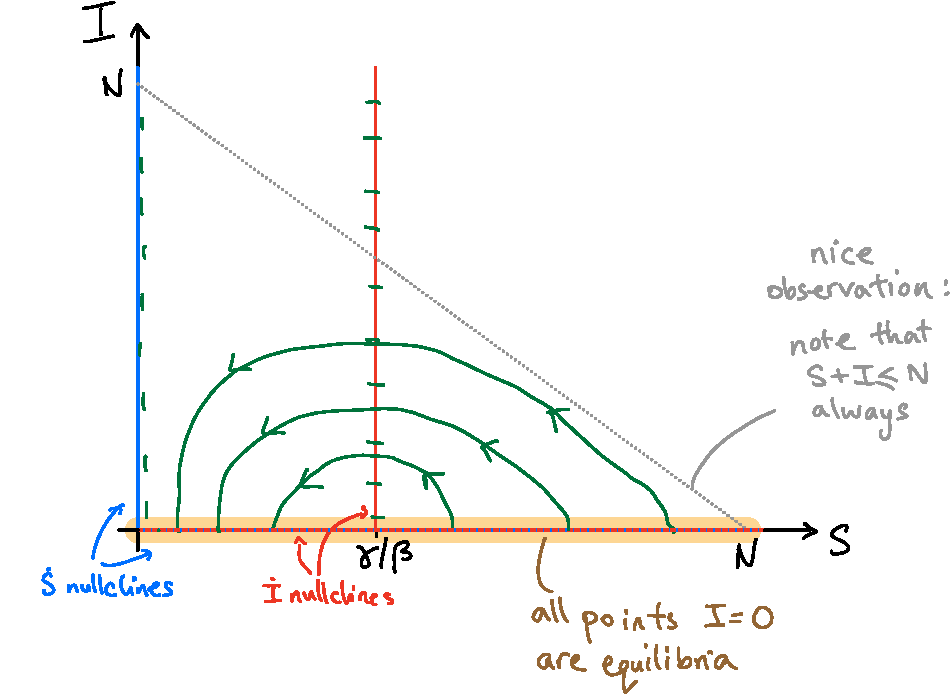
\includegraphics[width=0.9\textwidth]{images/sir-phase}
          \end{center}
          Equilibria are all along the like $I=0$: the first time we've seen this. Equilibria to the left of the $\dot{I}$ nullcline are stable; to the right, unstable.

        \item First note that $S$ is bounded above by $N$ (you can't have more susceptible people than people). If the $\dot{I}$ nullcline is to the right of $N$, then $I$ is decreasing in the entire permissible space, i.e.\ the disease is dying out. What does it mean for the nullcline to be to the right of $N$? It means
          \begin{equation}
            \gamma/\beta > N \implies N/R_0 > N \implies R_0 < 1,
          \end{equation}
          which is what we already knew from Problems class 1, but this time we see it graphically.

        \item
          \begin{enumerate}[label=(\roman*)]
            \item With no other information, we could assume that the number of patients requiring hospitalisation is a proportion of those who are infected, $I$.
            \item We look for when $\fd{I}{t} = 0$, i.e.\
              \begin{equation}
                0 = I(\beta S - \gamma).
              \end{equation}
              The maximum (assuming that it is a maximum, of course) occurs when $S = \gamma/\beta$.

            \item We get
              \begin{equation}
                \fd{I}{S} = \frac{\beta IS - \gamma I}{-\beta I S} = -1 + \frac{\gamma}{\beta S}.
              \end{equation}
              Integrating, this gives us
              \begin{equation}
                I = -S + \frac{\gamma}{\beta}\log S + C,
              \end{equation}
              where our initial condition of $I=I_0$, $S=N-I_0$ gives us that
              \begin{align}
                C &= I_0 + N - I_0 - \frac{\gamma}{\beta}\log (N-I_0),\\
                &= N - \frac{\gamma}{\beta}\log (N-I_0).
              \end{align}
              The maximum occurs when $S = \gamma/\beta$, giving us
              \begin{equation}
                I_{\text{max}} = - \frac{\gamma}{\beta} + \frac{\gamma}{\beta} \log\frac{\gamma}{\beta} + N - \frac{\gamma}{\beta} \log (N-I_0).
              \end{equation}
              Substituting in $R_0 = \beta N / \gamma$,
              \begin{align}
                I_{\text{max}} &= - \frac{N}{R_0} + \frac{N}{R_0} \log \frac{N}{R_0} + N - \frac{N}{R_0} \log (N-I_0) \\
                &= N\left[1 - \frac{1}{R_0}\left(1-\log \frac{N/R_0}{N-I_0}\right)\right].
              \end{align}
              If $I_0\ll N$, we are left with
              \begin{align}
                I_{\text{max}}&= N\left[1 - \frac{1+\log R_0}{R_0}\right].
              \end{align}
          \end{enumerate}
      \end{enumerate}

    }

    %Q2
    \question{SIR with temporary immunity}
    { % Question
      So far, we have assumed that immunity is permanent (how has this been encoded into our model?) What if immunity is only temporary? We know that Covid-19 reinfections are possible.
      \begin{enumerate}[label=(\alph*)]
        \item Introduce a new term to our equations which represents the `movement' of the population from the immune section, $R$, to the susceptible section, $S$.
        \item Show that there are two equilibria of this new model, with one of them given by
          \begin{equation}
            S = \frac{\gamma}{\beta}, \quad I = \frac{N-\frac{\gamma}{\beta}}{1 + \frac{\gamma}{\delta}}, \quad R = \frac{N-\frac{\gamma}{\beta}}{1 + \frac{\delta}{\gamma}},
          \end{equation}
          where $\delta$ is the factor on your $R$ terms in the governing equations. Is this different to our original SIR model, and if so, how?
        \item By using the equation for $N$ to eliminate $R$ from your expression for $\fd{S}{t}$, write down two equations governing this system.
        \item By writing down the Jacobian of this reduced system where appropriate, perform a linear stability analysis on the equilibria you have found, and state under what conditions each equilibrium is asymptotically stable/unstable/degenerate. (Hint: you may find the rules about determinants and traces useful.)
        \item How might you explain this to the general public? (Assuming you are able to crop your slides to the correct aspect ratio.) [This last comment would have been considered humorous and topical in 2020; maybe you remember this...?]
      \end{enumerate}
    }
    { % Solution
      \begin{enumerate}[label=(\alph*)]
        \item Our new system is
          \begin{align}
            \fd{S}{t} &= - \beta I S + \delta R, \\
            \fd{I}{t} &= \beta I S - \gamma I, \\
            \fd{R}{t} &= \gamma I - \delta R, \\
            N &= S + I + R.
          \end{align}

        \item In looking for equilibria, we set $\fd{S}{t} = \fd{I}{t} = \fd{R}{t} = 0$:
          \begin{align}
            0 &= - \beta I S + \delta R, \label{s-eq} \\
            0 &= I (\beta S - \gamma), \label{i-eq}\\
            0 &= \gamma I - \delta R, \\
            N &= S + I + R.
          \end{align}
          \Cref{i-eq} tells us that one possibility is $I=0$, in which case it follows that $R=0$ and $S=N$ from the other equations: i.e.\ this is our disease-free equilibrium.

          It also gives us the other possibility that $S = \gamma/\beta$. In which case, replacing $R$ with $N - S - I$ = $N -\gamma/\beta - I$ in \cref{s-eq} gives us
          \begin{align}
            0 &= -\beta I \frac{\gamma}{\beta} + \delta\left(N-\frac{\gamma}{\beta} - I\right)\\
            &= -I\gamma + \delta\left(N-\frac{\gamma}{\beta} - I\right) \\
            &= -I(\gamma+\delta) + \delta\left(N-\frac{\gamma}{\beta}\right),
          \end{align}
          i.e.\
          \begin{equation}
            I = \frac{\delta(N-\gamma/\beta)}{\gamma+\delta} = \frac{N-\frac{\gamma}{\beta}}{1 + \frac{\gamma}{\delta}}.
          \end{equation}

          Then,
          \begin{align}
            R &= N - S - I \\
            &= N - \frac{\gamma}{\beta} - \frac{\delta(N - \frac{\gamma}{\beta})}{\gamma+\delta} \\
            &= \frac{N(\gamma+\delta)-\frac{\gamma}{\beta}(\gamma+\delta)-\delta(N-\frac{\gamma}{\beta})}{\gamma+\delta} \\
            &= \frac{N\gamma - \gamma^2/\beta}{\gamma+\delta} = \frac{N-\frac{\gamma}{\beta}}{1 + \frac{\delta}{\gamma}}.
          \end{align}

          This is different to our original SIR model because although the disease-free equilibrium is the same, we don't have an additional one-parameter family of equilibria.

        \item As instructed,
          \begin{align}
            \fd{S}{t} &= - \beta I S + \delta(N - S - I),\\
            \fd{I}{t} &= \beta I S - \gamma I.
          \end{align}
          The Jacobian, $\m{J}$, is
          \begin{equation}
            \m{J} =
            \begin{pmatrix}
              -(\beta I + \delta) & -(\beta S + \delta) \\
              \beta I & \beta S - \gamma
            \end{pmatrix}.
          \end{equation}

        \item Linear stability analysis: on our disease-free equilibrium, $(S,I,R) = (N,0,0)$, our Jacobian is
          \begin{equation}
            \m{J} =
            \begin{pmatrix}
              -\delta & -(\beta N + \delta) \\
              0 & \beta N - \gamma
            \end{pmatrix}.
          \end{equation}
          Since there is a zero on the off-diagonal, the eigenvalues are just the terms on the diagonal, namely
          %Doing this the hard way (not looking at the trace/determinant), we see that solving $\det(\m{J} - \lambda\m{I}) = 0$ gives us
          \begin{equation}
            \lambda_1 = -\delta, \quad \lambda_2 = \beta N - \gamma.
          \end{equation}
          The second eigenvalue is only positive when $\beta N /\gamma > 1$, i.e.\ $R_0 > 1$, in which case this is \emph{unstable}. If $R_0 < 1$, it is \emph{asymptotically stable}.

          [If you did this the trace/determinant way---and you shouldn't, because the eigenvalues can be read off directly---you would get
            \begin{equation}
              \tr(\m{J}) = \beta N - \gamma -\delta, \qquad \det(\m{J}) = -\delta(\beta N-\gamma).
            \end{equation}
            The requirement for stability of positive determinant and negative trace means
            \begin{align}
              \det(\m{J})>0 \implies & \beta N - \gamma < 0,\\
              \tr(\m{J})<0 \implies & \beta N - \gamma - \delta < 0,
            \end{align}
          but since the bottom condition is weaker than the top, we just have $\beta N-\gamma<0$, i.e.\ $R_0 < 1$ for asymptotic stability.]

          As for the other equilibrium where $S = \gamma/\beta$, no off-diagonal zeros so we go for the trace/determinant approach directly:
          \begin{align}
            \tr(\m{J}) &= -(\beta I + \delta) + \beta S - \gamma \\
            &= -(\beta I + \delta)
          \end{align}
          which is negative because $\beta$, $I$ and $\delta$ are all positive terms. As for the determinant,
          \begin{align}
            \det(\m{J}) &= -(\beta I + \delta)(\beta S - \gamma) + (\beta S + \delta)\beta I \\
            &= (\gamma + \delta)\beta I
          \end{align}
          which is positive because it consists of purely positive terms. Since stability requires positive determinant and negative trace, this equilibrium is \emph{asymptotically stable}.

        \item (I leave this up to you)

      \end{enumerate}

    }

    % Q3
    \question{Advection and diffusion}
    {
      Last week we introduced the advection--diffusion equation for a concentration or population $c(\v{x},t)$,
      \begin{equation}
        \pd{c}{t} = -\vnabla\cdot(c\v{v})+D\Lap c + f.
      \end{equation}
      \begin{enumerate}[label=(\alph*)]
        \item In words, what is diffusion?
        \item In words, what is advection?
        \item What does $f$ represent?
        \item What does this equation look like in one spatial dimension, $\v{x}=x$?
      \end{enumerate}
    }
    { % Solution
      These questions are here just to solidify your intuition.
      \begin{enumerate}[label=(\alph*)]
        \item (for example) Diffusion is the spreading out of the population over space, essentially due to individual random motion (but the centre of mass stays the same).
        \item (for example) Advection is the movement of the centre of mass of the population, or in other words a bulk motion (think ducks being carried away down a river).
        \item $f(c)$ is any source or sink term, and this can be any of the population models we have seen so far this term.
        \item In one spatial dimension, this is
          \begin{equation}
            \pd{c}{t} = -\pd{}{x}(cv)+D\pdd{c}{x} + f.
          \end{equation}
      \end{enumerate}

    }

    %\section{SIR with natural birth and death}
    %We now return to our original SIR model, but add in natural birth and death. We haven't added this in so far (why might that be OK?) but don't forget that these terms also represent immigration and emigration: a rush of Londoners travelling to their second homes in Cornwall, for example.
    %\begin{enumerate}[label=(\alph*)]
    %  \item Add new terms to the original SIR system to model this new situation. (Be careful: natural death affects everybody!)
    %  \item In order to have a constant population ($\fd{N}{t} = 0$), what must we assume about the birth and death rates?
    %  \item Find the equilibria of this new model, and compare these to the models we have found so far.
    %  \item By considering the sub-system consisting of the equations for $\fd{S}{t}$ and $\fd{I}{t}$, once again write down the Jacobian and perform a linear stability analysis on these equilibria. What is $R_0$ in this new model?
    %\end{enumerate}
    %
    %\section{SEIR models}
    %For many diseases, there is an incubation period where the individual is infect\emph{ed} but not yet infect\emph{ious}.
    %\begin{enumerate}[label=(\alph*)]
    %  \item Keeping the natural birth and death terms from your previous model, add in a new class $E$ for the `exposed' population, so that the population goes through the process in the order
    %  \[ S \to E \to I \to R.\]
    %  \item Show that in this model, the basic reproduction number $R_0$ is given by
    %  \begin{equation}
    %    R_0 = \frac{\alpha\beta}{(\mu+\alpha)(\mu+\gamma)},
    %  \end{equation}
    %  where $\mu$ is the birth/death rate, $\alpha$ is your $E$ rate, $\beta$ is your $SI$ rate, and $\gamma$ is your $I$ rate.
    %\end{enumerate}
    %%Next time... vaccines.

\end{enumerate}
\end{document}
